%%%%%%%% ICML 2022 EXAMPLE LATEX SUBMISSION FILE %%%%%%%%%%%%%%%%%

\documentclass[nohyperref]{article}

% Recommended, but optional, packages for figures and better typesetting:
\usepackage{microtype}
\usepackage{graphicx}
\usepackage{subfigure}
\usepackage{booktabs} % for professional tables

% hyperref makes hyperlinks in the resulting PDF.
% If your build breaks (sometimes temporarily if a hyperlink spans a page)
% please comment out the following usepackage line and replace
% \usepackage{icml2022} with \usepackage[nohyperref]{icml2022} above.
\usepackage{hyperref}
\usepackage{lipsum}


% Attempt to make hyperref and algorithmic work together better:
\newcommand{\theHalgorithm}{\arabic{algorithm}}

% Use the following line for the initial blind version submitted for review:
\usepackage[accepted]{icml2022}

% If accepted, instead use the following line for the camera-ready submission:
% \usepackage[accepted]{icml2022}

% For theorems and such
\usepackage{amsmath}
\usepackage{amssymb}
\usepackage{mathtools}
\usepackage{amsthm}

% if you use cleveref..
\usepackage[capitalize,noabbrev]{cleveref}

%%%%%%%%%%%%%%%%%%%%%%%%%%%%%%%%
% THEOREMS
%%%%%%%%%%%%%%%%%%%%%%%%%%%%%%%%
\theoremstyle{plain}
\newtheorem{theorem}{Theorem}[section]
\newtheorem{proposition}[theorem]{Proposition}
\newtheorem{lemma}[theorem]{Lemma}
\newtheorem{corollary}[theorem]{Corollary}
\theoremstyle{definition}
\newtheorem{definition}[theorem]{Definition}
\newtheorem{assumption}[theorem]{Assumption}
\theoremstyle{remark}
\newtheorem{remark}[theorem]{Remark}

% Todonotes is useful during development; simply uncomment the next line
%    and comment out the line below the next line to turn off comments
%\usepackage[disable,textsize=tiny]{todonotes}
\usepackage[textsize=tiny]{todonotes}


% The \icmltitle you define below is probably too long as a header.
% Therefore, a short form for the running title is supplied here:
\icmltitlerunning{Counterfactual explanations of neural network predictions}

\begin{document}

\twocolumn[
\icmltitle{Generative counterfactual explanations of neural network predictions: \\ A Galactic Center Excess case study}

% It is OKAY to include author information, even for blind
% submissions: the style file will automatically remove it for you
% unless you've provided the [accepted] option to the icml2022
% package.

% List of affiliations: The first argument should be a (short)
% identifier you will use later to specify author affiliations
% Academic affiliations should list Department, University, City, Region, Country
% Industry affiliations should list Company, City, Region, Country

% You can specify symbols, otherwise they are numbered in order.
% Ideally, you should not use this facility. Affiliations will be numbered
% in order of appearance and this is the preferred way.
% \icmlsetsymbol{equal}{*}

\begin{icmlauthorlist}
\icmlauthor{Siddharth Mishra-Sharma}{IAIFI,MIT,Harvard}
\icmlauthor{Yitian Sun}{IAIFI,MIT}
\icmlauthor{Tracy Slatyer}{IAIFI,MIT}
\end{icmlauthorlist}

\icmlaffiliation{IAIFI}{The NSF AI Institute for Artificial Intelligence and Fundamental Interactions}
\icmlaffiliation{MIT}{Center for Theoretical Physics, Massachusetts Institute of Technology, Cambridge, MA 02139, USA}
\icmlaffiliation{Harvard}{Department of Physics, Harvard University, Cambridge, MA 02138, USA}

\icmlcorrespondingauthor{Siddharth Mishra-Sharma}{smsharma@mit.edu}

% You may provide any keywords that you
% find helpful for describing your paper; these are used to populate
% the "keywords" metadata in the PDF but will not be shown in the document
\icmlkeywords{Machine Learning, ICML}

\vskip 0.3in
]

% this must go after the closing bracket ] following \twocolumn[ ...

% This command actually creates the footnote in the first column
% listing the affiliations and the copyright notice.
% The command takes one argument, which is text to display at the start of the footnote.
% The \icmlEqualContribution command is standard text for equal contribution.
% Remove it (just {}) if you do not need this facility.

\printAffiliationsAndNotice{}  % leave blank if no need to mention equal contribution
% \printAffiliationsAndNotice{\icmlEqualContribution} % otherwise use the standard text.

\begin{abstract}
    \lipsum[1]
\end{abstract}

\section{Introduction}

The nature of the \emph{Fermi} $\gamma$-ray Galactic Center Excess (GCE) represents one of the enduring mysteries in astroparticle physics. Although the excess is broadly compatible with annihilating dark matter at the expected thermal cross-section, alternative explanations in terms of a population of astrophysics point sources (PSs), in particular millisecond pulsars, remain viable. Understanding the origin of the Excess is a challenging modeling and inference problem---the signal sits on top of a diffuse background of Galactic origin whose nature is subject to significant systematic uncertainties. The spatial morphology of the signal itself is contended, with a preference for dark matter or stellar origin exhibited depending on the details of the modeling.
  
Modeling the GCE including populations of unresolved point sources is challenging due to the large induced latent space representing the number and properties of individual point sources. Traditional likelihood-based methods therefore use a simplified representation of the problem, for example based on the counts probability distribution function (PDF) of the photon map or its wavelet decomposition. More recently, methods based on machine learning have been used to implicitly approximate the likelihood associated with the forward model using neural networks. By leveraging more information associated with the modeled data-generating process, these methods have been shown to be more robust to known systematic effects.

The robustness of a given method to systematic variations is generally tested by inducing a reasonable perturbation in simulated data away from the assumed model, then observing its response. This implicitly contains information about what kinds of systematic effects the model is sensitive to, and the kinds of biases they are likely to introduce.

In this paper, we propose an alternative approach to assessing the robustness of a neural network-based prediction of the composition of the GCE using procedurally-generating counterfactuals of the $\gamma$-ray data---data perturbations that have a desired predictive outcome---under a given predictive model. Since the data is known to not be accurately captured by the forward model, minimal counterfactuals can provide insight into the resiliency of the prediction---if small and reasonable data perturbations can lead to large variations in the predicted outcome, the results may be considered suspicious. Additionally, counterfactuals have significant explanatory power, since data features that modify the predicted contribution of a given modeled component to the $\gamma$-ray are indicative of the features that the neural network is using to drive its decisions for that component.

\section{Methodology}

\subsection{Data and inference model}

\lipsum[1-3]

\subsection{Normalizing flows for counterfactual generation}

%
\begin{figure*}
    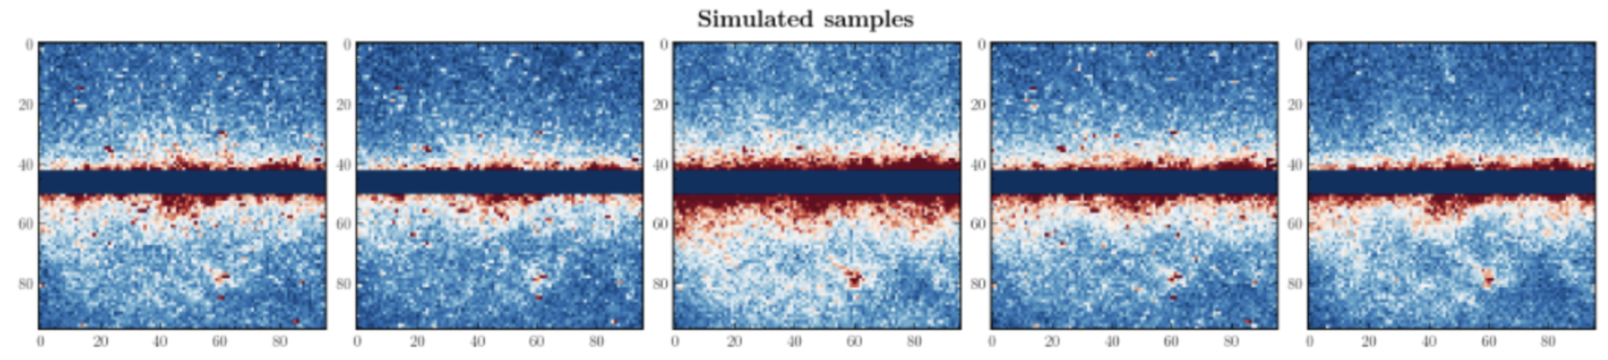
\includegraphics[width=0.95\textwidth]{figures/placeholder_1_1.png} \\
    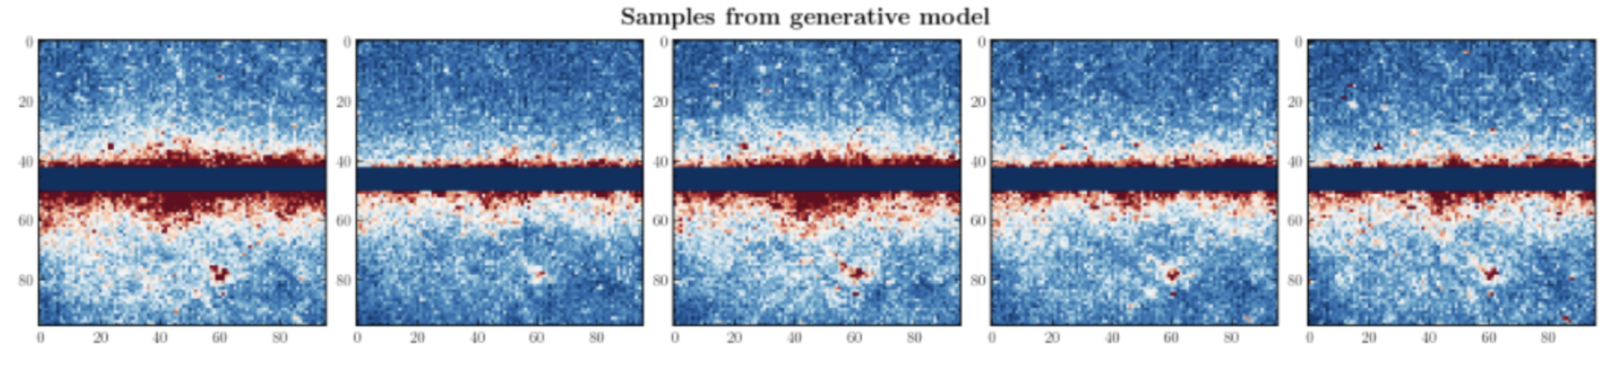
\includegraphics[width=0.95\textwidth]{figures/placeholder_1_2.png}
    \caption{\lipsum[1]}
    \label{fig:fid_data}
\end{figure*}
%

\paragraph*{Diffeomorphic counterfactuals}
Given a differentiable inference network $s(x)$ that predicts the contributions of different modeled components to the GCE, for example through the Gaussian means $s(x)_i \equiv \mu_i$ and log-variances $\log\sigma_i^2$, a straightforward way of constructing counterfactuals for a given component, indexed by $i$, is by performing gradient ascent on the data space starting from the dataset of interest $x^{0} = x$,
\begin{equation}
    x^{t+1}=x^{t}+\lambda \frac{\partial \left[s(x^{t})\right]_i}{\partial x},
\end{equation}
where $\lambda$ is a specified learning rate. Continuing to take gradient steps until a desired condition is achieved, for example when the predicted mean increases by at least one standard deviation $s(x^{t})_i > \mu_i + \sigma_i$, giving a \emph{minimal} counterfactual.

This scheme can be used to generate \emph{adversarial} counterfactuals of the map, \emph{i.e.} the minimal perturbations in $\mathbb R^{N_\mathrm{pix}}$ that change the predicted outcome in a desired way. Although they can be useful, such perturbations may not be physically meaningful or plausible, given some expectation for the ensemble of possible models. 

Instead, we leverage generative modeling with normalizing flows to construct counterfactuals that fall within a pre-defined distribution of models $p(x)$. Normalizing flows are a class of models that define bijective invertible transformations (\emph{diffeomorphisms}) $f: U\rightarrow X$ from a base distribution $\pi_{U}(u)$ that is easy to sample from and evaluate the probability density on, to a more complex target distribution $p_{X}(x)$. The transformation is usually parameterized by neural networks such that its Jacobian is numerically tractable, allowing for efficient density estimation and generative sampling. The flow defines a probability density in the target space through the inverse Jacobian determinant, ${p}_X(x)=\pi_U(u)\left|\operatorname{det}\left({\partial u}/{\partial x}\right)\right|=\pi_U\left(f^{-1}(x)\right)\left|\operatorname{det} J_{f^{-1}}(x)\right|$.

\begin{equation}
    u^{t+1}=u^{t}+\lambda \frac{\partial\left[s\left(f(u^{t})\right)\right]_{i}}{\partial u}
\end{equation}

As shown in \citet{dombrowski2021diffeomorphic}, performing gradient ascent in the base space $U$ ensures that, as long as the learning rate is small, the corresponding push forward $x^t=f(z^t)$ after each gradient update stays on the data manifold $X$ defined by $x\sim p_X(x)$. This allows us to construct physically-meaningful counterfactuals for a given $\gamma$-ray map.

\paragraph*{Generative model for Galactic Center $\gamma$-ray data}
We use an instantiation of the \texttt{Glow} normalizing flow architecture~\cite{DBLP:conf/nips/KingmaD18} to train a generative model the the Galactic Center $\gamma$-ray data. \texttt{Glow} is multi-scale normalizing flow architecture specialized for image synthesis and manipulation tasks. We configure the flow with $L=5$ layers of $K=18$ steps each and 256 channels.


\subsection{Counterfactual analyses of $\gamma$-ray maps}

\lipsum[1-2]

\begin{equation}
    \mathcal L = s\left(f(u^{t})\right)
\end{equation}

\begin{equation}
    \mathcal L = s\left(f(u^{t})\right)_i + \frac{1}{N_\mathrm{comp} - 1}\sum_j \left| s\left(f(u^{t})\right)_{j\neq i} - s(x^0)_{j\neq i} \right|
\end{equation}

\section{Tests on simulated data}

\lipsum[1-4]

%
\begin{figure*}
    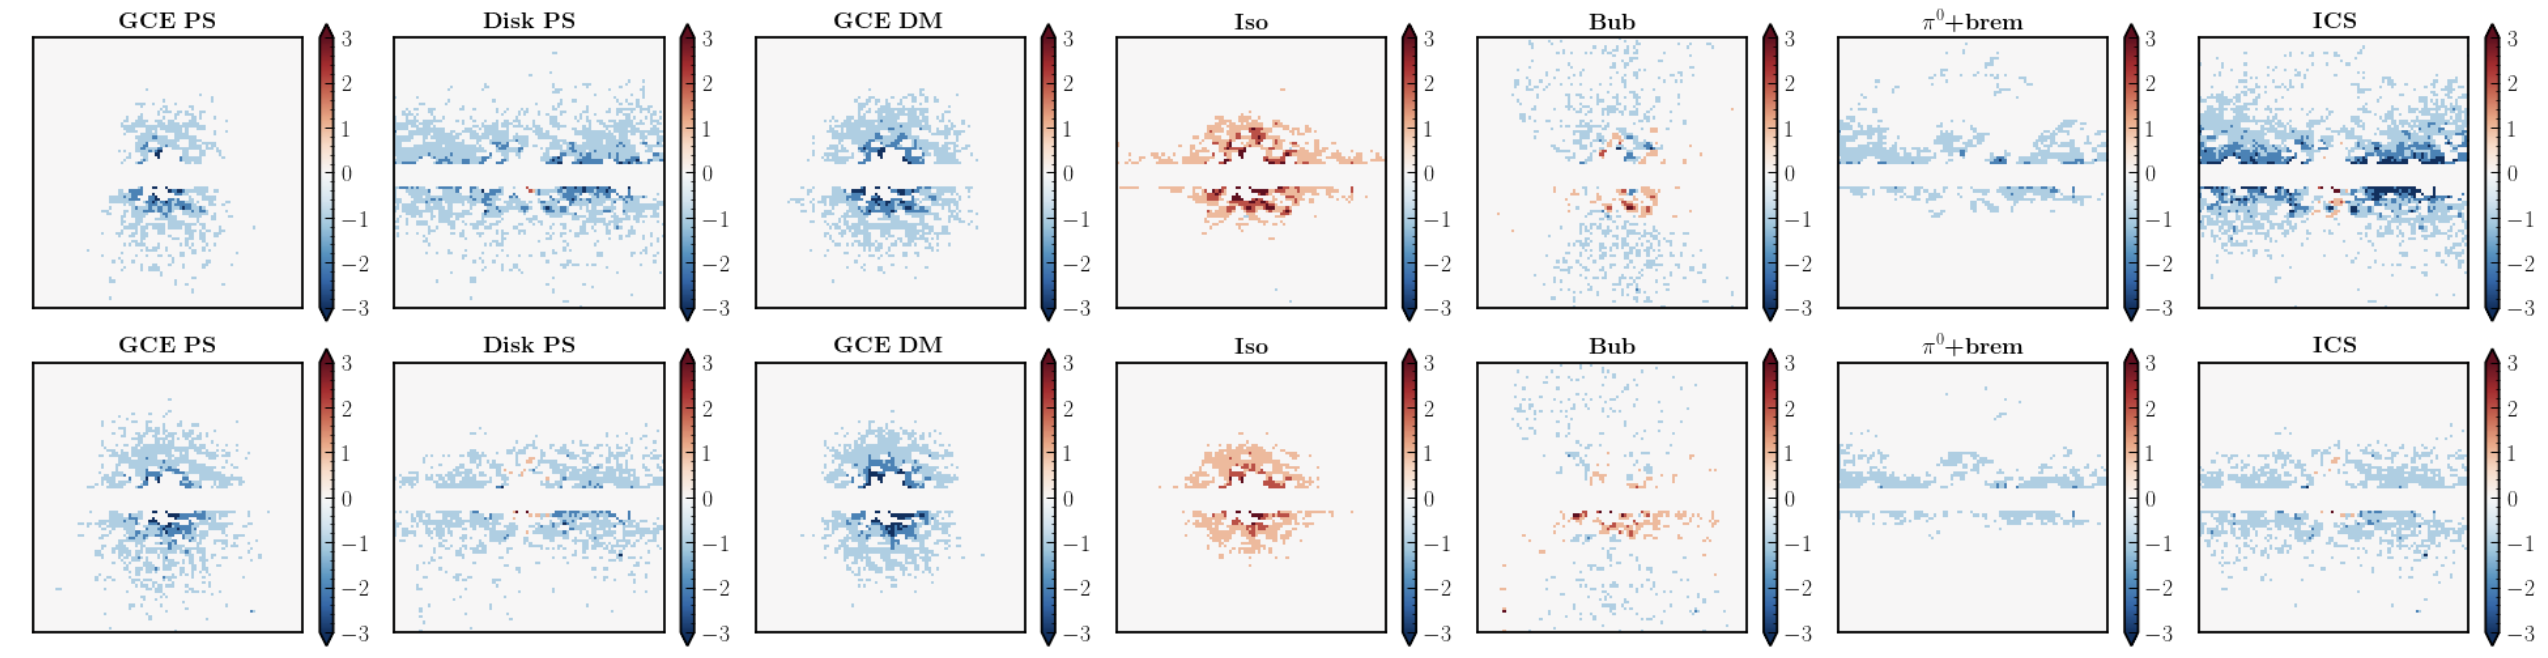
\includegraphics[width=0.95\textwidth]{figures/placeholder_2.png}
    \caption{\lipsum[1]}
    \label{fig:fid_data_2}
\end{figure*}
%

\section{Discussion and conclusions}

\lipsum[1-3]

\section*{Software and Data}

% Acknowledgements should only appear in the accepted version.
\section*{Acknowledgements}

\bibliography{fermi-counterfactuals}
\bibliographystyle{icml2022}


% %%%%%%%%%%%%%%%%%%%%%%%%%%%%%%%%%%%%%%%%%%%%%%%%%%%%%%%%%%%%%%%%%%%%%%%%%%%%%%%
% %%%%%%%%%%%%%%%%%%%%%%%%%%%%%%%%%%%%%%%%%%%%%%%%%%%%%%%%%%%%%%%%%%%%%%%%%%%%%%%
% % APPENDIX
% %%%%%%%%%%%%%%%%%%%%%%%%%%%%%%%%%%%%%%%%%%%%%%%%%%%%%%%%%%%%%%%%%%%%%%%%%%%%%%%
% %%%%%%%%%%%%%%%%%%%%%%%%%%%%%%%%%%%%%%%%%%%%%%%%%%%%%%%%%%%%%%%%%%%%%%%%%%%%%%%
% \newpage
% \appendix
% \onecolumn
% \section{You \emph{can} have an appendix here.}

% You can have as much text here as you want. The main body must be at most $8$ pages long.
% For the final version, one more page can be added.
% If you want, you can use an appendix like this one, even using the one-column format.
% %%%%%%%%%%%%%%%%%%%%%%%%%%%%%%%%%%%%%%%%%%%%%%%%%%%%%%%%%%%%%%%%%%%%%%%%%%%%%%%
% %%%%%%%%%%%%%%%%%%%%%%%%%%%%%%%%%%%%%%%%%%%%%%%%%%%%%%%%%%%%%%%%%%%%%%%%%%%%%%%


\end{document}


% This document was modified from the file originally made available by
% Pat Langley and Andrea Danyluk for ICML-2K. This version was created
% by Iain Murray in 2018, and modified by Alexandre Bouchard in
% 2019 and 2021 and by Csaba Szepesvari, Gang Niu and Sivan Sabato in 2022. 
% Previous contributors include Dan Roy, Lise Getoor and Tobias
% Scheffer, which was slightly modified from the 2010 version by
% Thorsten Joachims & Johannes Fuernkranz, slightly modified from the
% 2009 version by Kiri Wagstaff and Sam Roweis's 2008 version, which is
% slightly modified from Prasad Tadepalli's 2007 version which is a
% lightly changed version of the previous year's version by Andrew
% Moore, which was in turn edited from those of Kristian Kersting and
% Codrina Lauth. Alex Smola contributed to the algorithmic style files.
